\section{Results and interpretation}
\label{sec:results}

\subsection{Q2: Classification algorithms}
\inputtable{q2_grid_LogReg}
\inputtable{q2_grid_NaiveBayes}
\inputtable{q2_grid_kNN}
\inputtable{q2_summary}
\inputtable{q2_per_class}
\fig{q2_confusion_matrices}{Validation confusion matrices of the Q2 models.}
\fig[0.9]{q2_roc_pr}{ROC and precision--recall curves on validation.}

% TODO(student): interpret
\studenttodo{Q2a--c: compare the models (why NB representation X won; effect of $k$, weights, $p$; effect of
$C$ and class weighting); which metric is most useful for this dataset and why (accuracy vs.\ Macro-F1 vs.\
PR-AUC under 11.7\% prevalence); compare ROC-AUC and PR-AUC rankings.}

\subsection{Q2d: Class imbalance}
\inputtable{q2_imbalance}
\inputtable{q2_threshold_summary}
\fig[0.7]{q2_threshold_sweep}{Threshold sweep: OOF training and validation F1 as a function of the decision threshold.}

% TODO(student): interpret
\studenttodo{Q2d: class-wise errors with and without each intervention; does aggregate accuracy conceal
failures (compare Dummy and the no-intervention LogReg: high accuracy, low recall for \textit{yes})?
Trade-off between recall(yes) and precision(yes); is the threshold choice transferable?}

\subsection{Q3: Regression}
\inputtable{q3_audit}
\inputtable{q3_target_cap}
\inputtable{q3_high_corr_pairs}
\fig[0.6]{q3_target_hist}{Target distribution (training rows); note the cap at 5.0.}
\fig[0.65]{q3_corr_heatmap}{Correlation matrix (training rows).}
\inputtable{q3_model_comparison}
\fig{q3_complexity_curves}{Training vs.\ CV-validation RMSE as a function of model complexity.}
\inputtable{q3_complexity_curves}
\fig[0.65]{q3_learning_curves}{Learning curves.}

% TODO(student): interpret
\studenttodo{Q3a--c: target distribution and cap; correlated predictors and outliers; compare models
(Dummy vs.\ linear vs.\ non-linear); explain the complexity and learning curves with the bias--variance
framework (where under-/over-fitting starts).}

\fig{q3_coef_paths}{Ridge and Lasso coefficient paths (standardised features).}
\begin{figure}[H]\centering
\IfFileExists{figures/q3_cv_alpha_Ridge.pdf}{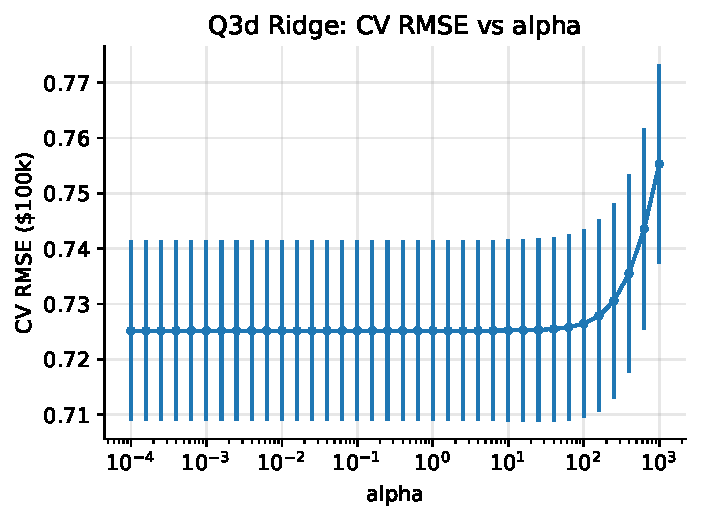
\includegraphics[width=0.45\linewidth]{figures/q3_cv_alpha_Ridge.pdf}}{}
\IfFileExists{figures/q3_cv_alpha_Lasso.pdf}{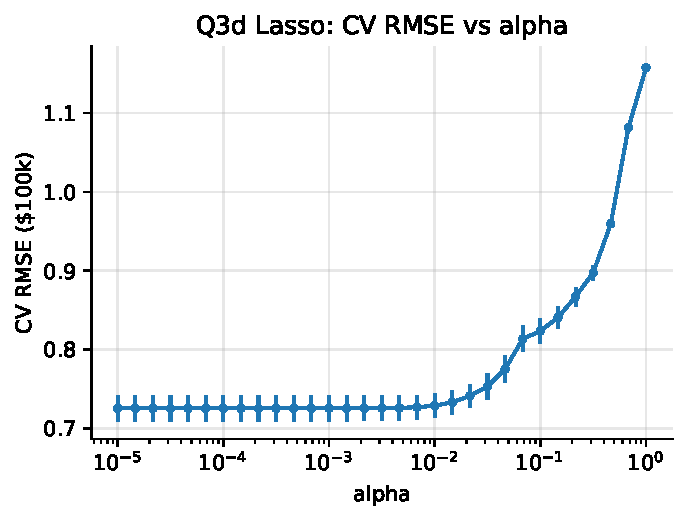
\includegraphics[width=0.45\linewidth]{figures/q3_cv_alpha_Lasso.pdf}}{}
\caption{CV RMSE vs.\ regularisation strength.}\end{figure}
\inputtable{q3_coefficients}
\inputtable{q3_sparsity}
\inputtable{q3_corr_coef_stability}

% TODO(student): interpret
\studenttodo{Q3d: shrinkage (Ridge) vs.\ sparsity (Lasso); why the CV-optimal $\alpha$ is small here (many
samples, few features); behaviour of the correlated pairs AveRooms/AveBedrms and Latitude/Longitude
(sign, magnitude, bootstrap instability).}

\fig{q3_residual_plots}{Predicted vs.\ actual and residuals vs.\ predicted on validation.}
\inputtable{q3_top_residuals}
\inputtable{q3_residual_by_band}

% TODO(student): interpret
\studenttodo{Q3e: interpret MAE/RMSE/R$^2$ in \$100k units; what the residual patterns suggest (capped
target at 5.0 $\Rightarrow$ systematic under-prediction; heteroscedasticity; unusual block groups such as very
high AveOccup); discuss at least five of the large residuals.}

\subsection{Q4: Decision trees, bagging, boosting}
\inputtable{q4_dt_criterion}
\inputtable{q4_dt_top10}
\inputtable{q4_dt_complexity}
\fig{q4_small_tree}{Depth-3 decision tree.}
\inputtable{q4_decision_paths}

% TODO(student): interpret
\studenttodo{Q4b: Gini vs.\ entropy (and log\_loss = entropy in sklearn, see \texttt{results/q4\_logloss\_check.json});
effect of each complexity control; interpret at least three decision paths in domain terms.}

\fig{q4_rf_curves}{Random Forest: training vs.\ validation Macro-F1.}
\inputtable{q4_rf_cv_results}
\inputtable{q4_rf_tree_correlation}
\fig[0.6]{q4_rf_tree_correlation}{Tree correlation vs.\ max\_features.}

% TODO(student): interpret
\studenttodo{Q4c: how bagging and random feature subsets reduce variance and tree correlation; trade-off
between single-tree strength and correlation; behaviour with number of trees and depth.}

\fig{q4_boosting_staged}{Boosting: staged training/validation Macro-F1 and CV grid vs.\ number of estimators.}
\inputtable{q4_AdaBoost_cv_top}
\inputtable{q4_GradientBoosting_cv_top}

% TODO(student): interpret
\studenttodo{Q4d: learning rate vs.\ number of estimators; sequential error correction (boosting reduces bias)
vs.\ independent bagged learners (variance reduction); effect of balanced sample weights. Note that the
CV-optimal n\_estimators lies at the upper end of the grid (see the CV tables) -- discuss what this implies.}

\inputtable{q4_comparison}
\inputtable{q4_importance_rank_corr}
\inputtable{q4_importance_RandomForest}
\inputtable{q4_importance_GradientBoosting}
\fig{q4_importances}{Built-in impurity importance vs.\ permutation importance on validation.}
\inputtable{q4_importance_control}
\fig{q4_importance_control}{Importance control experiment with added noise and near-duplicate features.}

% TODO(student): interpret
\studenttodo{Q4e: compare Macro-F1, accuracy, training and inference time; agreement between built-in and
permutation importance; at least two cases where importance misleads (impurity bias towards
high-cardinality/continuous features, importance split between correlated/duplicate features, importance
computed on training data, importance $\neq$ causality).}
